\documentclass[11pt]{article}
\usepackage{mypackages}
\begin{document}

% Max 

\section{Experiments}

The aim of this project is to examine the effect of asynchronous training
in Deep Reinforcement Learning.
To compare the aynchronous method, A3C, to a single-threaded approach,
we have implemented the Actor-Critic method with eligibility traces.
The results of this approach will work as a baseline for the
CartPole problem, as well as a proof of concept for Actor-Critic based
methods.
To measure the advantages and disadvantages of the A3C algorithm
compared to a single-threaded approach, we have also implemented this method
to solve the CartPole problem.
Both of the methods were allowed to perform the same amount of state transitions,
on a designated CPU cluster that consisted of 40 Intel Xeon E5-2670 2.5GHz CPUs.
This setting meant that we could be sure no one else could influence the results
of our experiments, since each experiment was assigned a number of CPUs
that only the experiment was allowed to use.

To further the test effect of different amounts of threads in the A3C algorithm,
we have also implemented the method in the more advanced setting of
games from the Atari 2600 system.
The experiments were performed on several \textbf{GPU} clusters, but only used 
the \textbf{CPUs} available on each cluster.
Unfortunately we weren't able to ensure the same controlled
setting as before, which means we can't be completely sure
no outside factors have influenced the final results.
Due to a lack of time we couldn't wait for the same cluster to
run all the experiments, so we have had to use different hardware
for some of the experiments.
The servers each consisted of 24 CPUs belonging to the Intel Xeon
E5-2600 series, with the subversions ranging from model E5-2620 to
E5-2695.

\subsection{Playing CartPole - Actor-Critic with eligibility traces}

For our first experiment we have implemented the Actor-Critic method
with eligibility traces as described in section \ref{sec:actor_critic_el}.
The pseudocode for the algorithm can be found in
appendix \ref{a:pseudo_code_et} and the a link to the actual
code can be found in appendix \ref{a:code}.
The goal of this experiment is to show that a 
traditional Reinforcement Learning algorithm
is able to learn how to solve the CartPole problem, as well as provide a
baseline performance for the A3C algorithm.
That is, as a measure to test if A3C is performing at least as good
as the single-threaded Actor-Critic approach.

For this experiment we used two separate neural networks, with no
shared weights, as policy and state-value estimators.
The network that estimated the state-value function consisted of an
input layer with four entries, corresponding to the format of a state in CartPole,
followed by a single hidden layer with eight neurons, and an output layer of a single
neuron.
We used a ReLU to activate the input to the
hidden layer and no activation for the output neuron.

For estimating the policy we used a network following the same architecture,
with the only exception being that the output layer consisted of two
neurons, each corresponding to the probability of picking an action.
To emulate a policy we used the softmax function
to activate the final layer.
For all of the experiments the networks were initialized with the same uniform
weights.

During the implementation of the algorithm, we occasionally encountered a problem with the
state-value network estimating a too large value.
This resulted in the policy and state-value estimates throwing a \texttt{NaN} error,
meaning they couldn't be represented using the bits they were assigned.
Therefore we had to restrict the parameters of the algorithm to
be small, which might cause the results of the
experiment being at a disadvantage, compared to our A3C implementation, since the learning
might happen at a slower pace than could be achieved with a better implementation.

\subsection{Playing CartPole - A3C}

To examine the effect of asynchronous training in the CartPole problem,
we have implemented the A3C algorithm discussed in section \ref{sec:a3c},
which we compare to the Actor-Critic method with eligibility traces.
The pseudo-code for the algorithm is given in appendix \ref{a:pseudo_code_a3c}
and a link to the actual code can be found in appendix \ref{a:code}.

We have chosen to also solve the CartPole problem using the A3C method, as a way to
investigate how asynchronous training influences the stability and performance of the algorithm,
compared to the more traditional Actor-Critic approach, as well as 
to itself with different amounts of threads.
We occasionally encountered the same \texttt{NaN} error as in the previous implementation,
but to a much lesser degree.
This means that the error should have little to no impact on
the final results.

To estimate the policy and state-value functions we used a single
neural network.
The structure of the network resembles the structure described in the previous section, 
with the key difference being that the network has two output layers -
one output layer for the policy and another for the value estimate.

\begin{figure}[H]
    \centering
    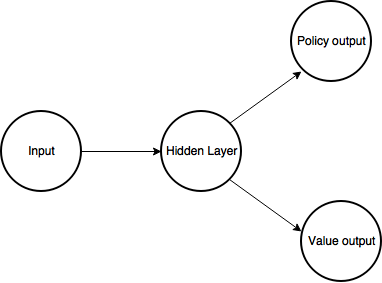
\includegraphics[scale=0.5]{include/shared_cartpole.png}
    \caption{The neural network used to estimate both the state-value
             and policy functions.}
    \label{fig:s_cartpole}
\end{figure}

For both the CartPole problem and the Atari games we will be using the same asynchronous setup
as described in \cite{a3c}.
This means that we use a single global network, whose only
purpose is to keep track of a set of global weights, and a local network
for each thread.
To perform the asynchronous update of the global weights we will be using
RMSProp as described in section \ref{sec:a3c}.
The parameters of the RMSProp, and the algorithm in general, have
been chosen because they provided decent test results during implementation
of the algorithm.
Due to the time limitations of the project we haven't performed
a more sophisticated selection of the parameters, which might
cause the experiments to learn at a suboptimal pace.

\subsection{Playing Atari Games}

To investigating how the asynchronous training performs in
a more advanced setting, we have also implemented the A3C algorithm
to play Atari games.
We will be examining the effect different amounts of threads
have on the performance and learning pace in the games Space Invader, Breakout
and Pong, as well as compare the results to those of the Cartpole experiment
where we also use the A3C method.

Taking an action in an Atari game leads to a relatively small state change,
since it is only performed for two to four frames.
To increase the impact of taking an action we have used the same \textit{action repeat}
stategy as described in \cite{a3c}, which means that an action is performed four times
after being sampled.
Instead of feeding the network a single frame from the games as a state,
we stack the four latest frames, such that the network may be able
to infer the movement of objects.
We also accumulate the rewards that we are given during the action repeat,
since they are all a product of performing that action.

For this experiment we used a single network with two separate
output layers as described in \cite{a3c}, with the exception that
the input layer of the network takes an $84 \times 84 \times 4$
image-stack as input.
This layer is followed by a convolutional layer that reduces the dimensions
of each element in the stack by a factor of four in both dimensions.
Using 16 kernel filters, the layer produces 16 different
$21 \times 21$ feature maps.
In the next layer the size of each of the 16 feature maps is
cut in half, by a convolution with stirdes, that produces 32 new feature maps consisting
of $11 \times 11$ values.
Both of the convolutional layers activates
their input using the ReLU function.
After the second convolution, we flatten the output.
We perform this step to allow the network to output a numerical value and
probability vector instead of a multichannel matrix.
The flattening of the last convolutional layer results in a new layer with $3872$ neurons,
that are fully connected to another layer with 256 neurons.
In this layer the input is again activated by a ReLU function,
and the output is sent to two different layers.
One of the layers consists of a single neuron
and simply outputs the weighted sum of its input as the estimated value
of the state.
The other output layer activates its input using the softmax function,
with as many neurons as actions available,
where output of each of the neurons represents the probability of taking an action.
A representation of the network is shown below.

\begin{figure}[H]
    \centering
    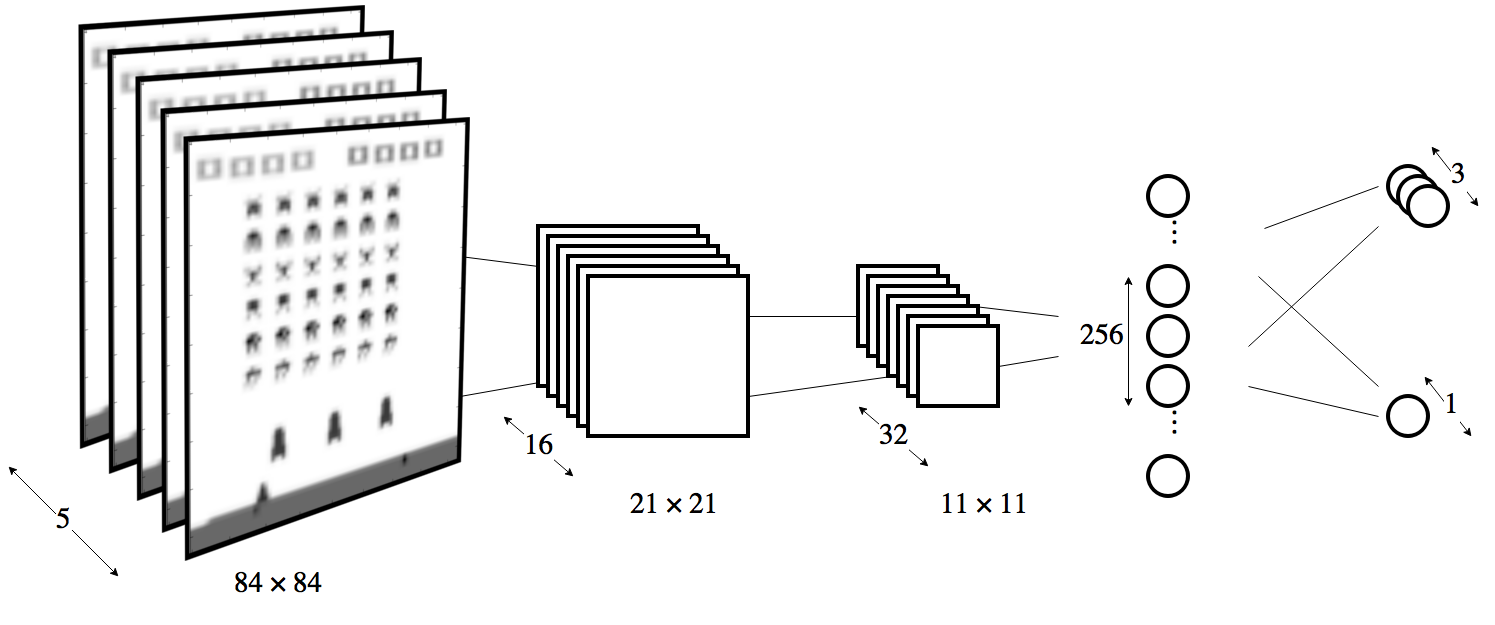
\includegraphics[scale=0.25]{include/Atari_network.png}
    \caption{The neural network used to estimate both the state-value
             and policy functions for Atari games. In this example the network
             is used on Space Invaders which means it has to assign each of three actions a probability.}
    \label{fig:atari_network}
\end{figure}

In Space Invaders we perform two additional preprocessing steps before
the states are fed to the network.
The obtainable rewards vary based on which aliens the learning agent
hits.
However, we want the learning agent to learn to shoot all aliens in a level,
and not focus on only shooting the ones that produce the greatest reward.
Therefore we have chosen to alter the rewards returned by the environment, such that
shooting an alien always yields reward one, which we expect will increase
the pace of learning.
The other issue in Space Invaders is that the screen sometimes flicker,
which can cause the frame to be missing some objects.
To avoid this issue we define a state as the pixel-wise maximum
between the last and second-to-last frame of the action repeat.

\end{document}
